\documentclass[serif]{beamer}\usepackage[]{graphicx}\usepackage[]{color}
%% maxwidth is the original width if it is less than linewidth
%% otherwise use linewidth (to make sure the graphics do not exceed the margin)
\makeatletter
\def\maxwidth{ %
  \ifdim\Gin@nat@width>\linewidth
    \linewidth
  \else
    \Gin@nat@width
  \fi
}
\makeatother

\definecolor{fgcolor}{rgb}{0.345, 0.345, 0.345}
\newcommand{\hlnum}[1]{\textcolor[rgb]{0.686,0.059,0.569}{#1}}%
\newcommand{\hlstr}[1]{\textcolor[rgb]{0.192,0.494,0.8}{#1}}%
\newcommand{\hlcom}[1]{\textcolor[rgb]{0.678,0.584,0.686}{\textit{#1}}}%
\newcommand{\hlopt}[1]{\textcolor[rgb]{0,0,0}{#1}}%
\newcommand{\hlstd}[1]{\textcolor[rgb]{0.345,0.345,0.345}{#1}}%
\newcommand{\hlkwa}[1]{\textcolor[rgb]{0.161,0.373,0.58}{\textbf{#1}}}%
\newcommand{\hlkwb}[1]{\textcolor[rgb]{0.69,0.353,0.396}{#1}}%
\newcommand{\hlkwc}[1]{\textcolor[rgb]{0.333,0.667,0.333}{#1}}%
\newcommand{\hlkwd}[1]{\textcolor[rgb]{0.737,0.353,0.396}{\textbf{#1}}}%

\usepackage{framed}
\makeatletter
\newenvironment{kframe}{%
 \def\at@end@of@kframe{}%
 \ifinner\ifhmode%
  \def\at@end@of@kframe{\end{minipage}}%
  \begin{minipage}{\columnwidth}%
 \fi\fi%
 \def\FrameCommand##1{\hskip\@totalleftmargin \hskip-\fboxsep
 \colorbox{shadecolor}{##1}\hskip-\fboxsep
     % There is no \\@totalrightmargin, so:
     \hskip-\linewidth \hskip-\@totalleftmargin \hskip\columnwidth}%
 \MakeFramed {\advance\hsize-\width
   \@totalleftmargin\z@ \linewidth\hsize
   \@setminipage}}%
 {\par\unskip\endMakeFramed%
 \at@end@of@kframe}
\makeatother

\definecolor{shadecolor}{rgb}{.97, .97, .97}
\definecolor{messagecolor}{rgb}{0, 0, 0}
\definecolor{warningcolor}{rgb}{1, 0, 1}
\definecolor{errorcolor}{rgb}{1, 0, 0}
\newenvironment{knitrout}{}{} % an empty environment to be redefined in TeX

\usepackage{alltt}
\usetheme{Boadilla}
\usepackage{graphicx}
\usepackage[final]{animate}
\usepackage{breqn}
\usepackage{xcolor}
\usepackage{booktabs}
\usepackage{tikz}
\usetikzlibrary{decorations.pathreplacing}
\usetikzlibrary{shapes,arrows,positioning,shadows}
\usepackage{subfig}
\usepackage{pgf}
\usepackage{caption}

% change format of enumerated lists
\setbeamertemplate{enumerate items}[default]
\setbeamertemplate{navigation symbols}{}

% change font size for figure captions
\setbeamerfont{caption}{size=\scriptsize}

% custom colors
\definecolor{mypal1}{HTML}{F0F9E8}\definecolor{mypal2}{HTML}{BAE4BC}\definecolor{mypal3}{HTML}{7BCCC4}\definecolor{mypal4}{HTML}{43A2CA}\definecolor{mypal5}{HTML}{0868AC}

% title graphic


\tikzstyle{decision} = [diamond, draw, text width=6em, text badly centered, inner sep = 2pt, top color=white, bottom color=mypal3, drop shadow]
\tikzstyle{block} = [rectangle, draw, text width=10em, text centered, rounded corners, minimum height=3em, minimum width=8em, top color = white, bottom color=mypal4,  drop shadow]
\tikzstyle{declare} = [rectangle, draw, text width=10em, text centered, minimum height=3em, minimum width=8em, top color = white, bottom color=mypal5,  drop shadow]

% knitr setup


% dependent data


% get online bib file


% figure used on title page


\setbeamercolor{title}{fg=mypal5} % main title
\setbeamercolor{frametitle}{fg=mypal4, bg=mypal2} % frame titles
\setbeamercolor{structure}{fg=mypal4} % bottom banner
\setbeamercolor{normal text}{fg=mypal5}
\usebackgroundtemplate{
\includegraphics[height=\paperheight,width=\paperwidth]{fig/back_tmp.pdf}}

% macros
\newcommand{\emtxt}[1]{\textbf{\textit{#1}}}
\IfFileExists{upquote.sty}{\usepackage{upquote}}{}
\begin{document}

\title[Understanding nitrogen pollution]{\textbf{Quantitative approaches to understanding nitrogen pollution: Examples from the upper San Francisco Estuary}}
\author[M. Beck]{Marcus W. Beck, PhD}

\institute[USEPA]{USEPA National Health and Environmental Effects Research Laboratory, Gulf Ecology Division, \href{mailto:beck.marcus@epa.gov}{beck.marcus@epa.gov}, Phone: 8509342480}

\date{Aug. 26, 2016}

\titlegraphic{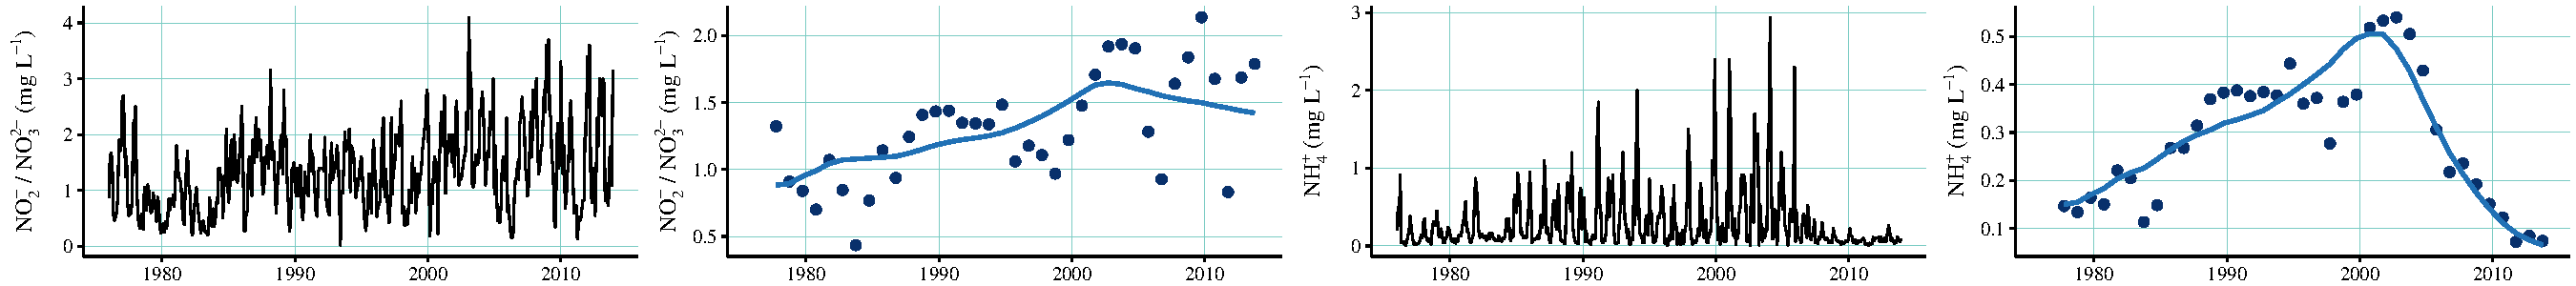
\includegraphics[width=\linewidth]{fig/titlegraphic.pdf}}

%%%%%%
\begin{frame}[shrink]
\vspace{0.2in}
\titlepage
\end{frame}

\section{Background}

%%%%%%
\begin{frame}{\textbf{Evaluating estuarine condition}}{\textbf{How do we collect and use data?}}
How can we leverage monitoring data to develop our conceptual model of eutrophication? \\~\\
\onslide<+->
\begin{quote}
Eutrophication (noun) - an \emtxt{increase} in the rate of supply of \emtxt{organic matter} to an ecosystem\\
\hfill -- \cite{Nixon95}
\end{quote}
\begin{center}
\scalebox{1}{
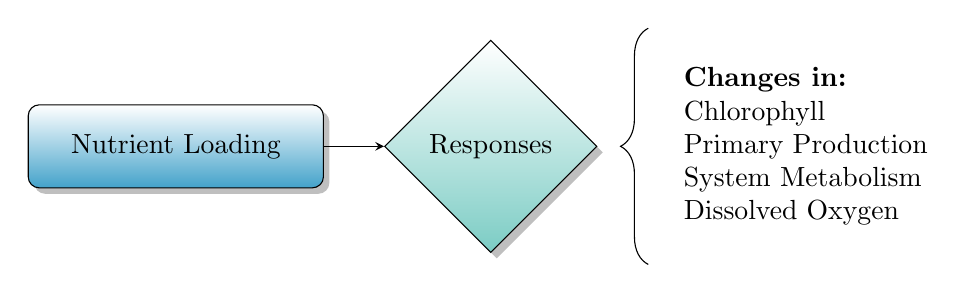
\begin{tikzpicture}[node distance = 4cm, auto, >=stealth]
  \onslide<+->{
  \node[block] (a) {Nutrient Loading};}
  \onslide<+->{
	\node[decision] (b)  [right of=a] {Responses};
 	\draw[->] (a) -- (b);}
  \onslide<+->{
  \draw[decorate,decoration={brace,amplitude=10pt}] [right of=b] (2,-1.5) -- (2,1.5);
  \node[draw,align=left,draw=none] [right of=b] {\textbf{Changes in:}\\ Chlorophyll\\ Primary Production\\ System Metabolism\\ Dissolved Oxygen};}
\end{tikzpicture}}
\end{center}
\vspace{-0.5cm}\hspace*{15pt}\scalebox{0.7}{\hbox{\tiny Adapted from \cite{Cloern01}}}\\~\\
\end{frame}

%%%%%%
\begin{frame}{\textbf{Evaluating estuarine condition}}{\textbf{How do we collect and use data?}}
\onslide<+->
\emtxt{Today's talk}: My experience evaluating monitoring data to inform our understanding of the eutrophication paradigm\\~\\
\onslide<+->
Water quality trends in the Delta: \\~\\
\begin{itemize}
\item \emtxt{Example 1}: Model theory and application \\~\\
\item \emtxt{Example 2}: Trends over time \\~\\
\item \emtxt{Example 3}: Selected case studies \\~\\
\end{itemize}
\onslide<+->
Can we \emtxt{develop} and \emtxt{apply} methods that \emtxt{link trends} with \emtxt{causal events}?
\end{frame}

\section{Model theory and background}



%%%%%%
\begin{frame}[t]{\textbf{Model theory and background}}{\textbf{WRTDS adaptation for tidal waters}}
{\bf \centerline{Observed data represents effects of many processes}}
\vspace{0.15in}
\centerline{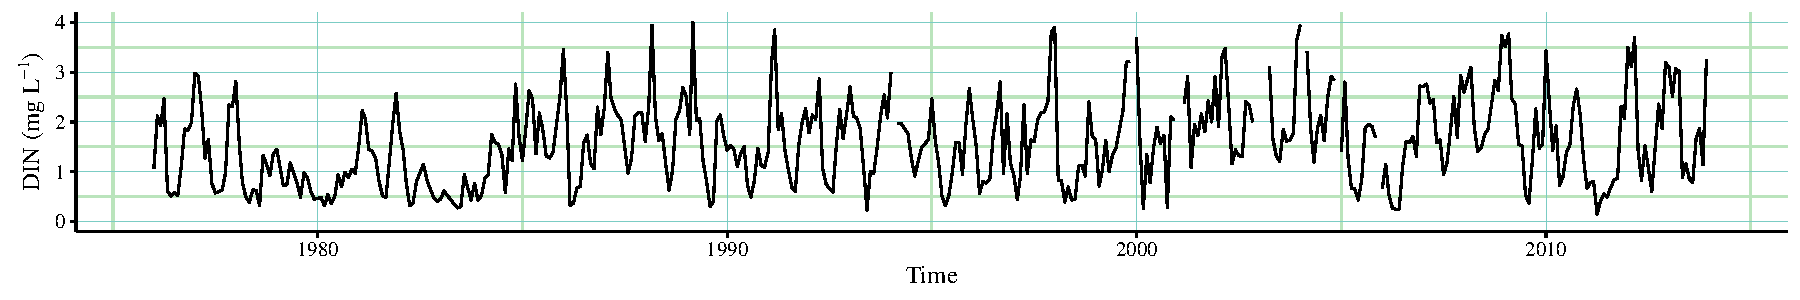
\includegraphics[width = \textwidth]{fig/ts_ex.pdf}}
\vspace{0.15in}
\begin{columns}[t]
\begin{column}{0.3\textwidth}
{\bf \underline{\emtxt{Climate}}}\\
precipitation\\
temperature\\
wind events\\
ENSO effects
\end{column}
\begin{column}{0.3\textwidth}
{\bf \underline{\emtxt{Local}}}\\
light/turbidity\\
residence time\\
invasive species\\
trophic effects
\end{column}
\begin{column}{0.3\textwidth}
{\bf \underline{\emtxt{Regional/historical}}}\\
watershed inputs\\
point sources\\
management actions
flow changes
\end{column}
\end{columns}
\end{frame}

%%%%%%
\begin{frame}[t]{\textbf{Model theory and background}}{\textbf{WRTDS adaptation for tidal waters}}
\onslide<+->
{\bf \centerline{Observed data represents effects of many processes}}
\vspace{0.15in}
\centerline{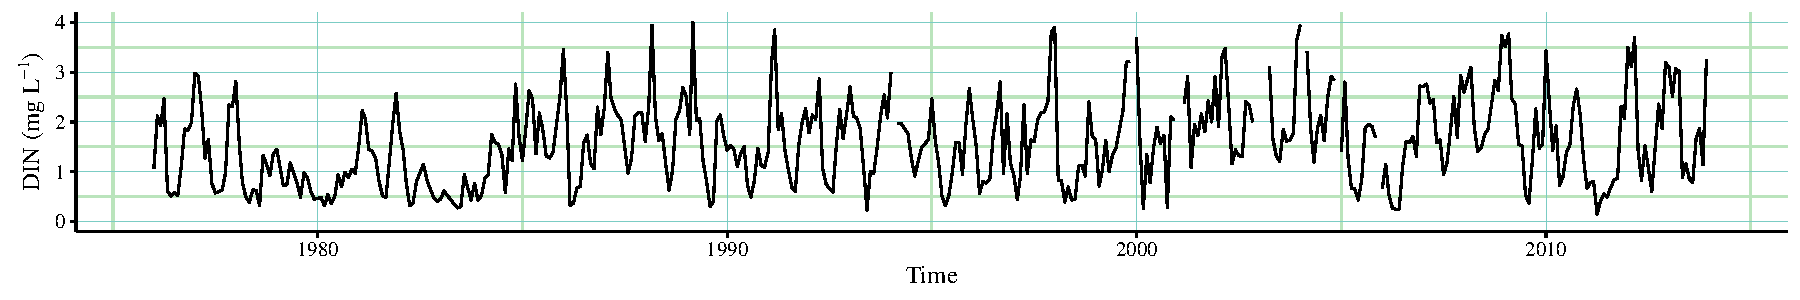
\includegraphics[width = \textwidth]{fig/ts_ex.pdf}}
\centerline{Models should describe components to evaluate effects}
\vspace{-0.1in}
\begin{columns}[t]
\begin{column}{0.5\textwidth}
\onslide<+->{
\centerline{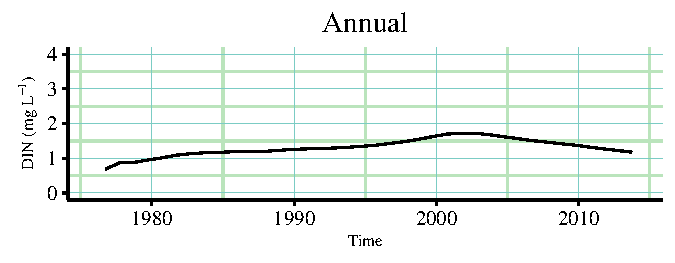
\includegraphics[width = 0.8\textwidth]{fig/schematic2.pdf}}
\centerline{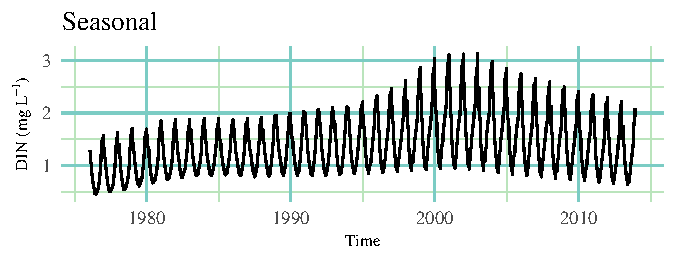
\includegraphics[width = 0.8\textwidth]{fig/schematic3.pdf}}
}
\end{column}
\begin{column}{0.5\textwidth}
\onslide<+->{
\centerline{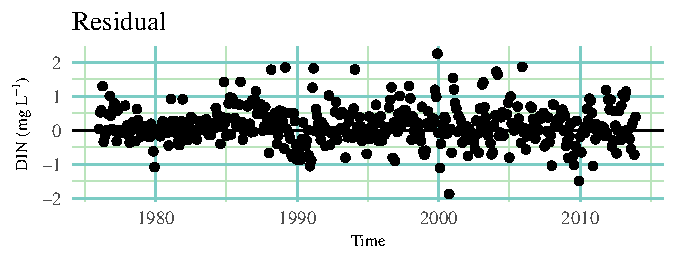
\includegraphics[width = 0.8\textwidth]{fig/schematic4.pdf}}
\centerline{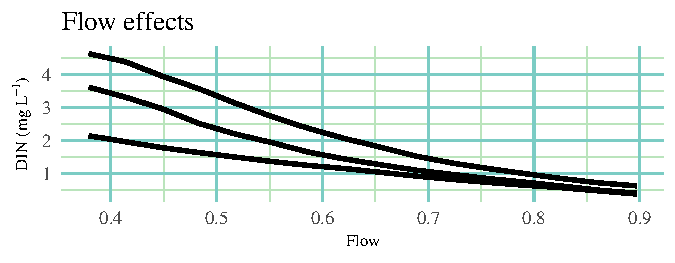
\includegraphics[width = 0.8\textwidth]{fig/schematic5.pdf}}
}
\end{column}
\end{columns}
\end{frame}

%%%%%%
\begin{frame}[t]{\textbf{Model theory and background}}{\textbf{WRTDS adaptation for tidal waters}}
\onslide<+->
\emtxt{Problem:} Response endpoints of eutrophication vary naturally over time and with discharge or tidal patterns\\~\\
\emtxt{Solution:} Develop a model that accounts for changes in relationships between drivers of pollution over time\\~\\
\onslide<+->
The \emtxt{weighted regression (WRTDS)} approach models pollutants in rivers as a function of \emtxt{time}, \emtxt{discharge}, and \emtxt{season} \cite{Hirsch10}\\~\\
\onslide<+->
\emtxt{Adaptation:} Applied to Tampa Bay \cite{Beck15}, further validated/compared in Patuxent Estuary [Beck and Murphy, In review]
\end{frame}



%%%%%%
\begin{frame}{\textbf{Model theory and background}}{\textbf{WRTDS adaptation for tidal waters}}
How does weighted regression work?
\begin{center}
\animategraphics[controls,width=\linewidth]{10}{fig/wtex}{}{} %frame rate is 12 per/sec
\end{center}
\end{frame}
 

 
%%%%%%
\begin{frame}{\textbf{Model theory and background}}{\textbf{WRTDS adaptation for tidal waters}} 
{\bf \centerline{Application to Delta}}
\begin{columns}
\begin{column}{0.45\textwidth}
\begin{itemize}
\item Nine stations (three Suisun, three middle, three delta) \\~\\
\item Three analytes (DIN, ammonium, nitrite/nitrate), two flow records \\~\\
\item Four decades of data, 1976-2013
\end{itemize}
\end{column}
\begin{column}{0.5\textwidth}
\begin{figure}
\begin{center}
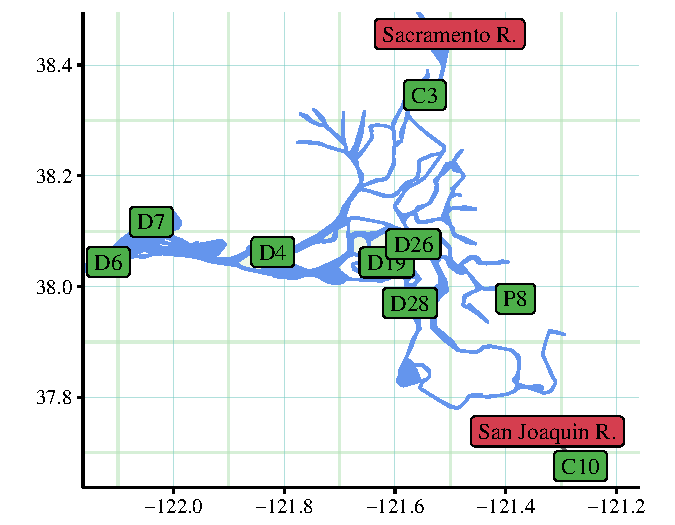
\includegraphics[width = \textwidth]{fig/stations.pdf}
\caption{Stations (green) and flow estimates (red) modelled with WRTDS}
\end{center}
\end{figure}
\end{column}
\end{columns}
\end{frame}

\section{Trends}



%%%%%%
\begin{frame}{\textbf{Trends over time}}{\textbf{Nitrogen dynamics in the Delta}} 
{\bf \centerline{Predicted DIN trends, 1980-1990}}
\vspace{0.05in}
\centerline{
\animategraphics[controls,width=\linewidth]{7}{fig/trnds}{}{} %frame rate is 10 per/sec
}
\end{frame}



%%%%%%
\begin{frame}{\textbf{Trends over time}}{\textbf{Nitrogen dynamics in the Delta - DIN}} 
\centerline{
\includegraphics[width = 0.93\textwidth, page = 2]{fig/trndsperdin.pdf}}
\end{frame}

%%%%%%
\begin{frame}{\textbf{Trends over time}}{\textbf{Nitrogen dynamics in the Delta - ammonium}} 
\centerline{
\includegraphics[width = 0.93\textwidth, page = 2]{fig/trndspernh.pdf}}
\end{frame}

%%%%%%
\begin{frame}{\textbf{Trends over time}}{\textbf{Nitrogen dynamics in the Delta - nitrite/nitate}} 
\centerline{
\includegraphics[width = 0.93\textwidth, page = 2]{fig/trndsperno23.pdf}}
\end{frame}



%%%%%%
\begin{frame}{\textbf{Trends over time}}{\textbf{Nitrogen dynamics in the Delta - nitrite/nitate}} 
The \emtxt{WRTDS} approach lets us model historical trends in relation to \emtxt{time}, \emtxt{discharge}, and \emtxt{season}\\~\\
Predicted trends follow observed... how can we leverage the results to better understand important processes? \\~\\
\centerline{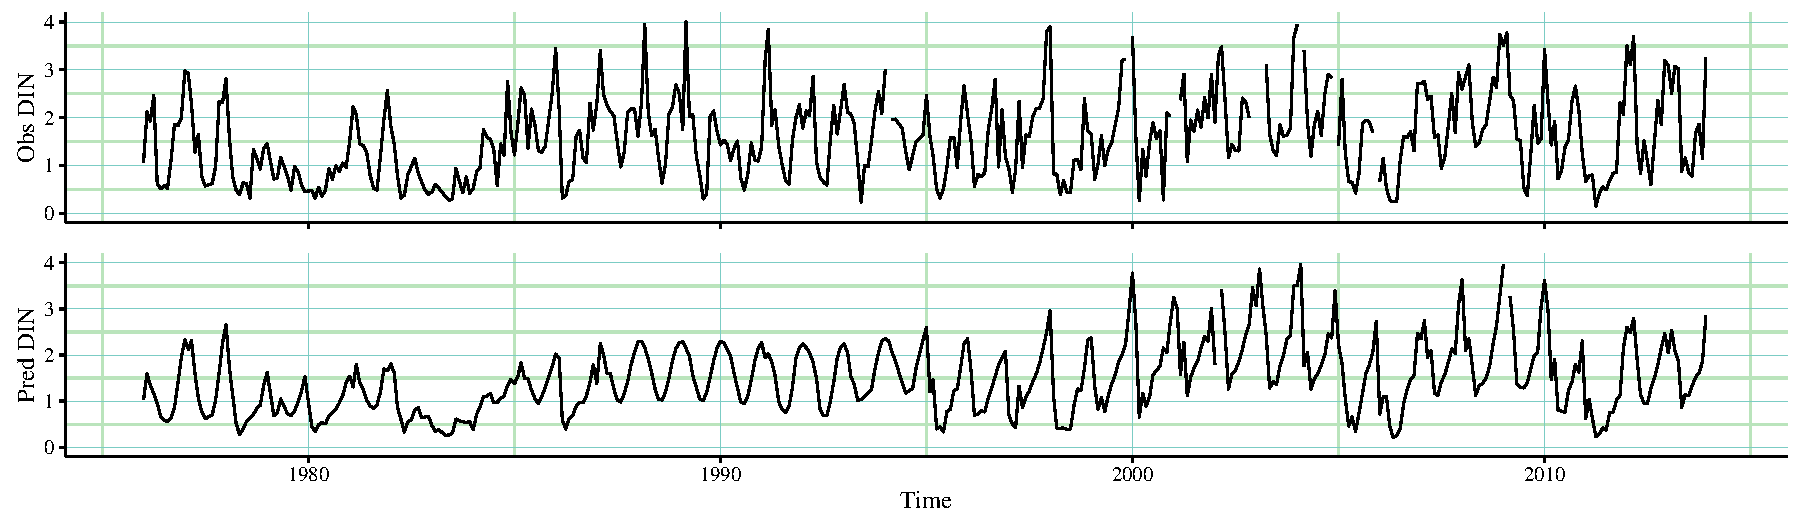
\includegraphics[width = \textwidth]{fig/ts_ex2.pdf}}
\end{frame}

\section{Selected case studies}

%%%%%%
\begin{frame}{\textbf{Selected case studies}}{\textbf{}}
\onslide<+->
Two examples demonstrate the utility of WRTDS adaptation to tidal waters: \\~\\
\begin{itemize}
\item Effects of wastewater treatment at P8 \\~\\
\item Effects of biological invasion in Suisun Bay\\~\\
\end{itemize}
\onslide<+->
Each shows how \emtxt{model components} describe \emtxt{processes}
\end{frame}



%%%%%%
\begin{frame}{\textbf{Selected case studies}}{\textbf{Effects of wastewater treatment upgrades}}
How can model information be linked to causation?
\vspace{0.1in}
\begin{figure}
\centerline{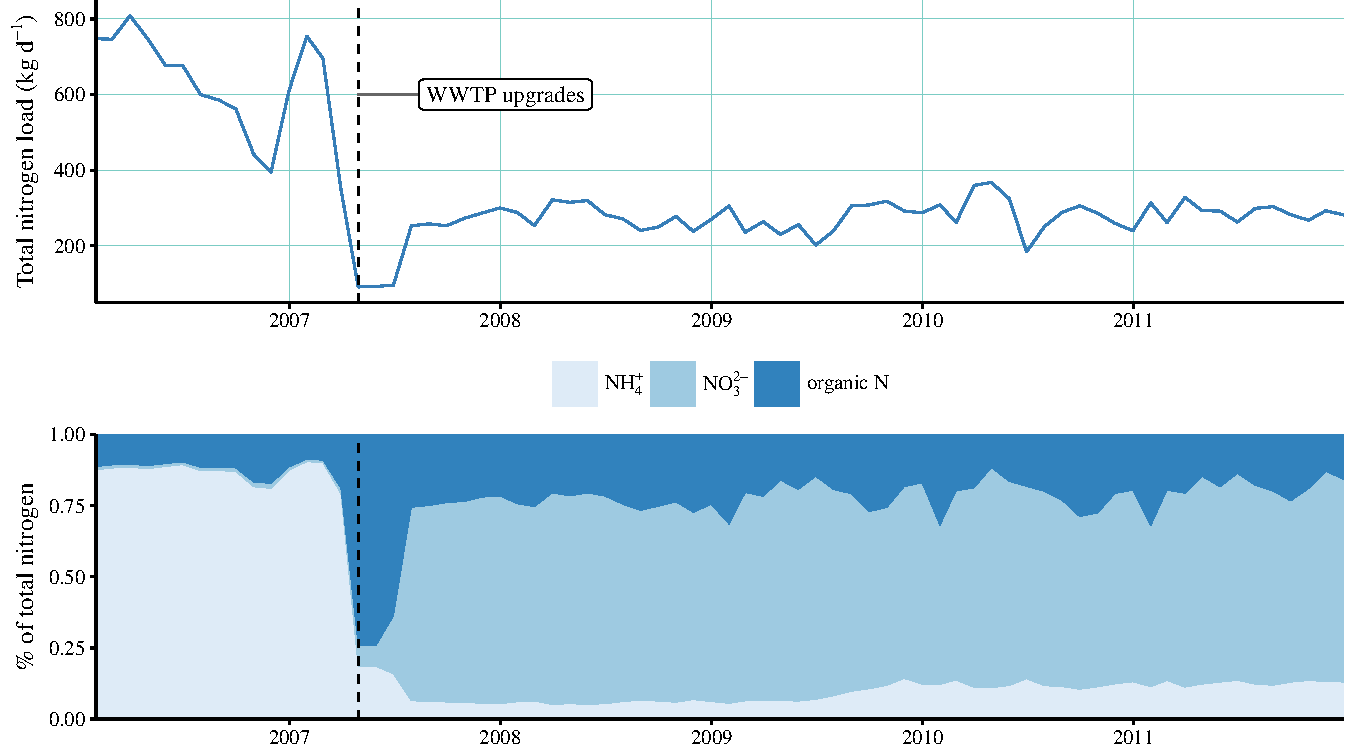
\includegraphics[width = 0.8\textwidth]{fig/tracy.pdf}}
\caption{Nitrogen load measurements (kg d$^{-1}$) at the Tracy Wastewater Treatment Plant.  Wastewater discharge requirements were implemented in May, 2007.}
\end{figure}
\end{frame}

%%%%%%
\begin{frame}{\textbf{Selected case studies}}{\textbf{Effects of wastewater treatment upgrades}}
\emtxt{Hypothesis}: Response of nutrient concentrations at P8 is linked to upstream WWTP upgrades \\~\\
We should be able to \emtxt{predict}: \\~\\
\begin{itemize}
\item A flow-normalized annual trend concurrent with WWTP upgrades \\~\\
\item Variation in nitrogen species response depending on change in load outputs
\end{itemize}
\end{frame}



%%%%%%
\begin{frame}{\textbf{Selected case studies}}{\textbf{Effects of wastewater treatment upgrades}}
\onslide<+->
\begin{figure}
\centerline{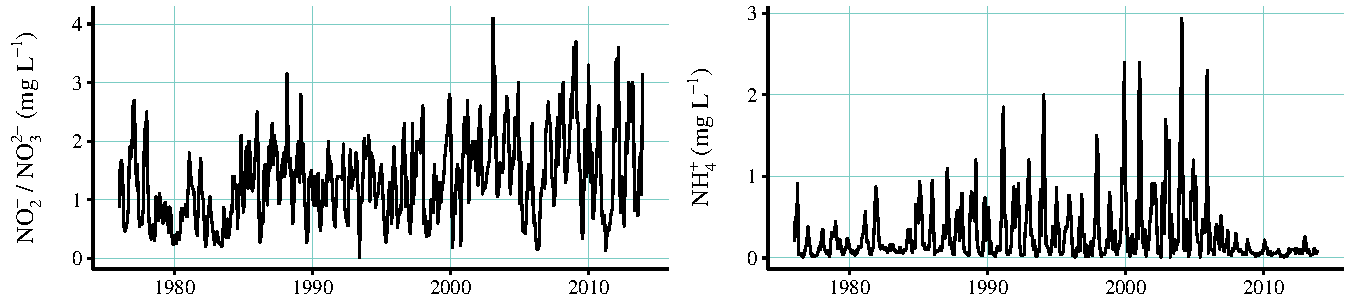
\includegraphics[width = \textwidth]{fig/p8obs.pdf}}
\caption{Observed nitrogen time series at P8}
\end{figure}
\onslide<+->
\vspace{-0.35in}
\begin{figure}
\centerline{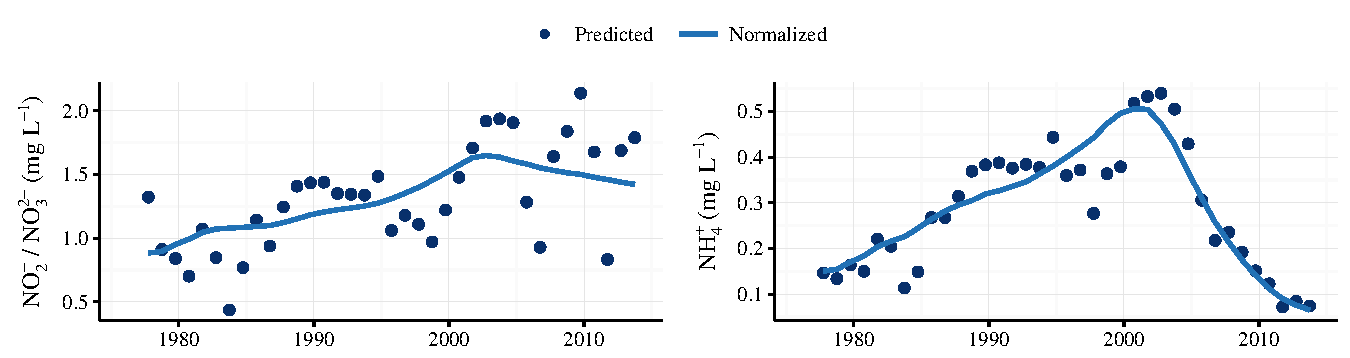
\includegraphics[width = \textwidth]{fig/p8prdnrm.pdf}}
\caption{Annual predicted and flow-normalized nitrogen from WRTDS.}
\end{figure}
\end{frame}

%%%%%%
\begin{frame}{\textbf{Selected case studies}}{\textbf{Effects of wastewater treatment upgrades}}
\vspace{0.1in}
\begin{figure}
\centerline{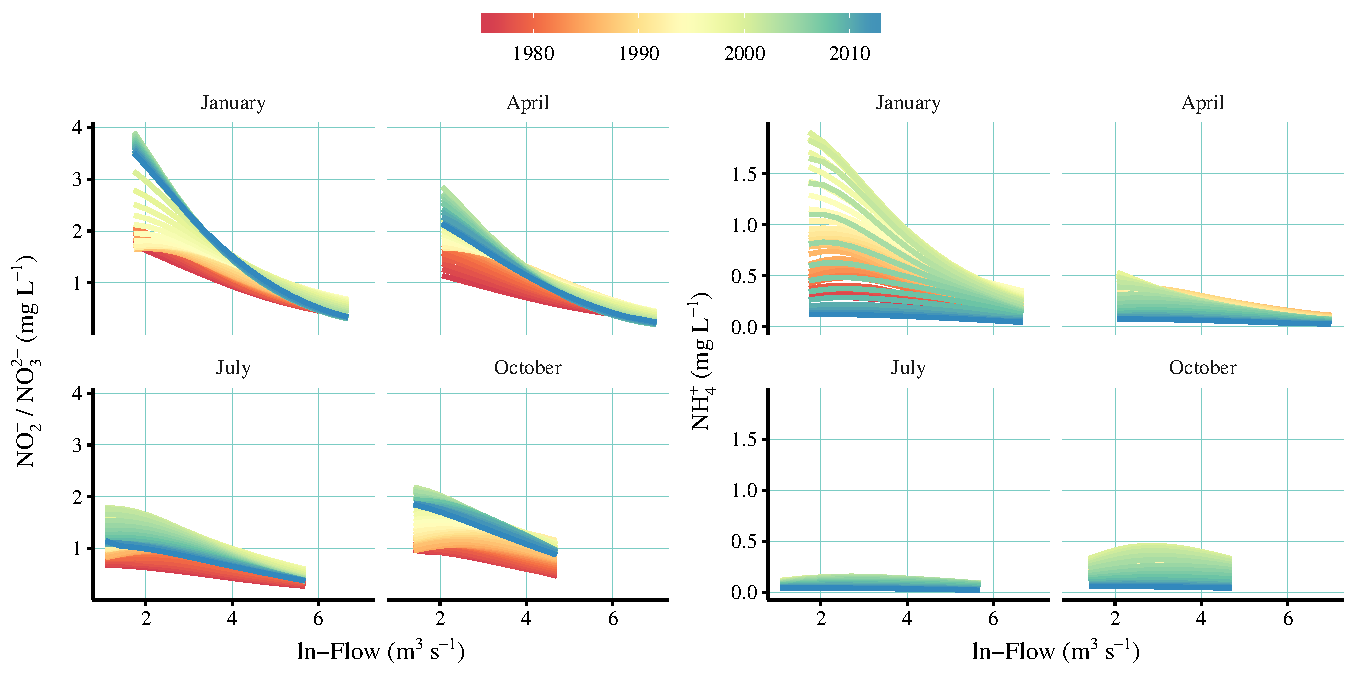
\includegraphics[width = \textwidth]{fig/p8dyna.pdf}}
\caption{Nitrogen relationships with flow over time at P8.}
\end{figure}
\end{frame}

%%%%%%
\begin{frame}{\textbf{Selected case studies}}{\textbf{Effects of wastewater treatment upgrades}}
Results at P8 were linked to WWTP upgrades:
\begin{columns}
\begin{column}{0.45\textwidth}
\begin{itemize}
\item Flow-normalized changes in ammonium, also nitrite/nitrate \\~\\
\item Ammonium reductions occurred in winter \\~\\
\item Largest response of ammonium at low flow... but not in summer
\end{itemize}
\end{column}
\begin{column}{0.4\textwidth}
\vspace{0.3in}
\centerline{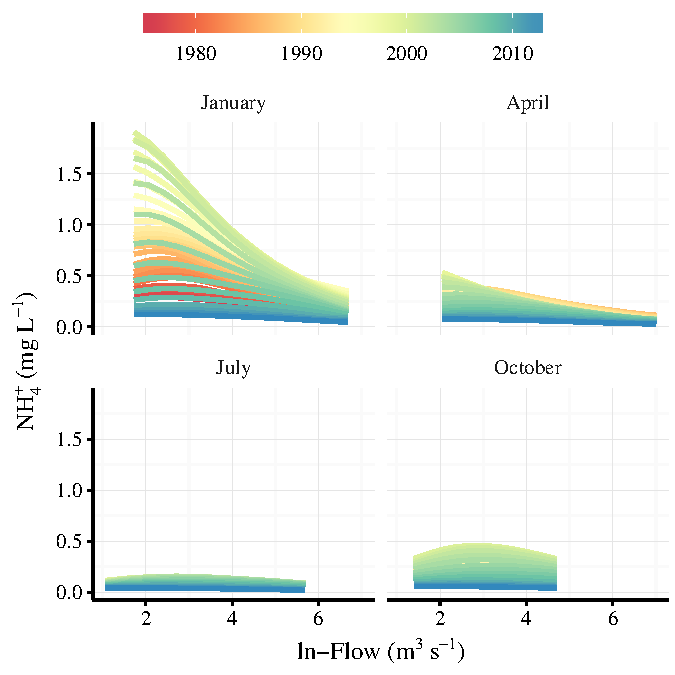
\includegraphics[width = \textwidth]{fig/p8dyna_thumb.pdf}}
\end{column}
\end{columns}
\end{frame}

%%%%%%
\begin{frame}{\textbf{Selected case studies}}{\textbf{Effects of biological invasion in Suisun Bay}}
\emtxt{Hypothesis}: Biological invasions by benthic filter feeders have shifted abundance and composition of phytoplankton in Suisun Bay \\~\\
We should be able to \emtxt{predict}: \\~\\
\begin{itemize}
\item A decline in annual, flow-normalized chlorophyll following increase in invaders\\~\\
\item Varying effects of flow given complex relationships between chlorophyll and invaders
\end{itemize}
\end{frame}



%%%%%%
\begin{frame}{\textbf{Selected case studies}}{\textbf{Effects of biological invasion in Suisun Bay}}
\vspace{-0.1in}
\onslide<1->
\begin{figure}
\centerline{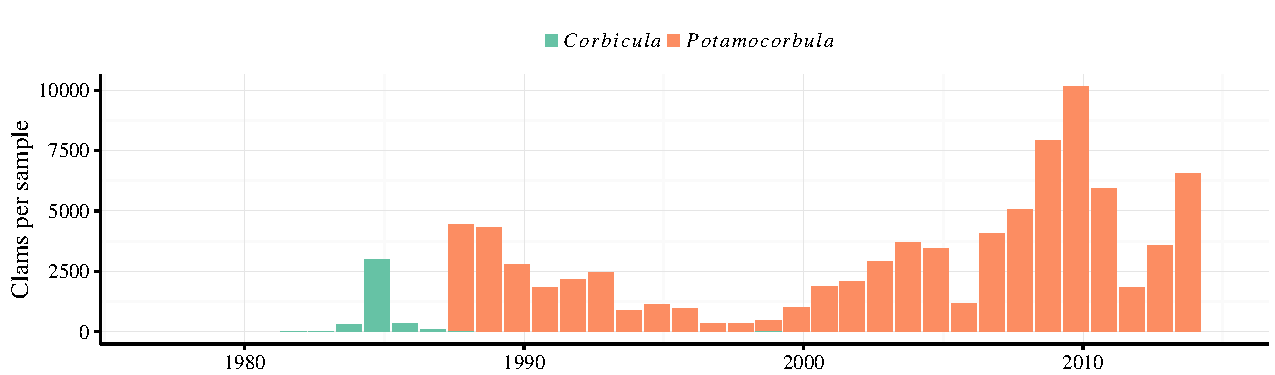
\includegraphics[width = \textwidth]{fig/d7clam.pdf}}
\caption{Clam density by year at D7, Suisun Bay \cite{Crauder16}.}
\end{figure}
\vspace{-0.1in}
\begin{columns}
\begin{column}{0.35\textwidth}
\onslide<2->{
\includegraphics[width = \textwidth, page = 2]{fig/d7prdnrm.pdf}
}
\end{column}
\begin{column}{0.35\textwidth}
\onslide<3->{
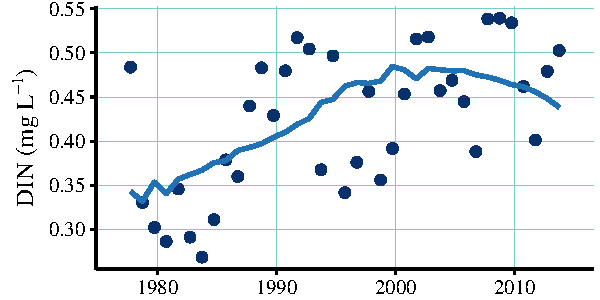
\includegraphics[width = \textwidth, page = 1]{fig/d7prdnrm.pdf}
}
\end{column}
\begin{column}{0.35\textwidth}
\onslide<4->{
\includegraphics[width = \textwidth, page = 3]{fig/d7prdnrm.pdf}
}
\end{column}
\end{columns}
\vspace{-0.05in}
\onslide<2->
\begin{figure}
\caption{Annual predicted (points) and flow-normalized (lines) water quality data at D7.}
\end{figure}
\end{frame}



%%%%%%
\begin{frame}{\textbf{Selected case studies}}{\textbf{Effects of biological invasion in Suisun Bay}}
\onslide<1->
\begin{columns}
\begin{column}{0.5\textwidth}
\centerline{\includegraphics[width = 0.95\textwidth, page = 3]{fig/d7flos.pdf}}
\end{column}
\begin{column}{0.5\textwidth}
\begin{itemize}
\item Early: Flow-stimulation, then flushing \\~\\
\item Later: Flow-stimulation
\end{itemize}
\end{column}
\end{columns}
\begin{columns}
\begin{column}{0.5\textwidth}
\onslide<2->{
\centerline{\includegraphics[width = 0.95\textwidth, page = 2]{fig/d7flos.pdf}}
}
\end{column}
\begin{column}{0.5\textwidth}
\onslide<3->{
\centerline{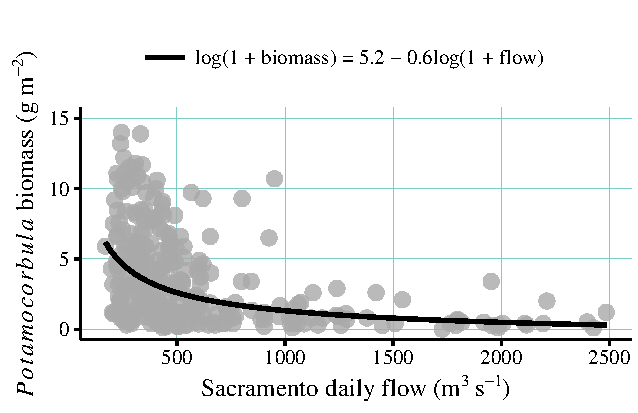
\includegraphics[width = 0.95\textwidth, page = 1]{fig/d7flos.pdf}}
}
\end{column}
\end{columns}
\end{frame}



%%%%%%
\begin{frame}{\textbf{Selected case studies}}{\textbf{Effects of biological invasion in Suisun Bay}}
\onslide<1->
\centerline{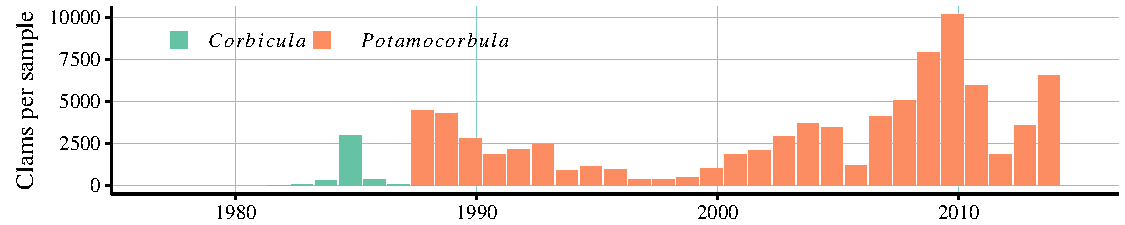
\includegraphics[width = 0.97\textwidth, page = 1]{fig/d7links.pdf}}
\onslide<2->
\centerline{\includegraphics[width = 0.97\textwidth, page = 2]{fig/d7links.pdf}}
\onslide<3->
\centerline{\includegraphics[width = 0.97\textwidth, page = 3]{fig/d7links.pdf}}
\end{frame}

%%%%%%
\begin{frame}[t]{\textbf{Selected case studies}}{\textbf{Effects of biological invasion in Suisun Bay}}
\onslide<1->
Results at D7 show complex response of chlorophyll:
\vspace{0.05in}
\begin{columns}[t]
\begin{column}{0.5\textwidth}
\vspace{0.2in}
\begin{itemize}
\onslide<1->{
\item Increase in clam abundance, decrease in chlorophyll \\~\\
\item Increase in DIN... but also increase in SiO$_2$ \\~\\
}
\onslide<2->{
\item Relationship with flow changed depending on physical or biological forcing
}
\end{itemize}
\end{column}
\begin{column}{0.25\textwidth}

\includegraphics<1>[width = \textwidth, trim = 0mm -10mm 0mm 0mm, clip, page = 2]{fig/d7prdnrm.pdf}

\includegraphics<1>[width = \textwidth, trim = 0mm -10mm 0mm 0mm, clip, page = 1]{fig/d7prdnrm.pdf}

\includegraphics<1>[width = \textwidth, trim = 0mm -10mm 0mm 0mm, clip, page = 3]{fig/d7prdnrm.pdf}
\includegraphics<2>[width = \textwidth, page = 3]{fig/d7flos.pdf}

\includegraphics<2>[width = \textwidth, page = 2]{fig/d7flos.pdf}

\includegraphics<2>[width = \textwidth, page = 1]{fig/d7flos.pdf}
\end{column}
\end{columns}
\end{frame}

\section{Conclusions and future work}

%%%%%%
\begin{frame}{\textbf{Conclusions}}{\textbf{Lessons for monitoring and future work}}
\onslide<+->
Monitoring data are not particularly telling... \\
...so we use models or other methods to \emtxt{decompose} the observations \\~\\
\onslide<+->
Chosen method depends on the question: WRTDS because water quality varies with time, season, and flow \\~\\
\onslide<+->
\begin{itemize}
\item More complete description of trends
\item Better link to causal events
\item More comprehensive evaluation of site-specific issues
\item Deconstruct the past to predict the future\\~\\
\end{itemize}
\onslide<+->
\emtxt{WRTDStidal} package for R, active development
\href{https://github.com/fawda123/WRTDStidal}{\url{https://github.com/fawda123/WRTDStidal}}
\end{frame}

% patux map


% patux trends


%%%%%%
\begin{frame}{\textbf{Conclusions}}{\textbf{Lessons for monitoring and future work}}
Comparing WRTDS and GAMs for trend evaluation
\begin{columns}
\begin{column}{0.38\textwidth}
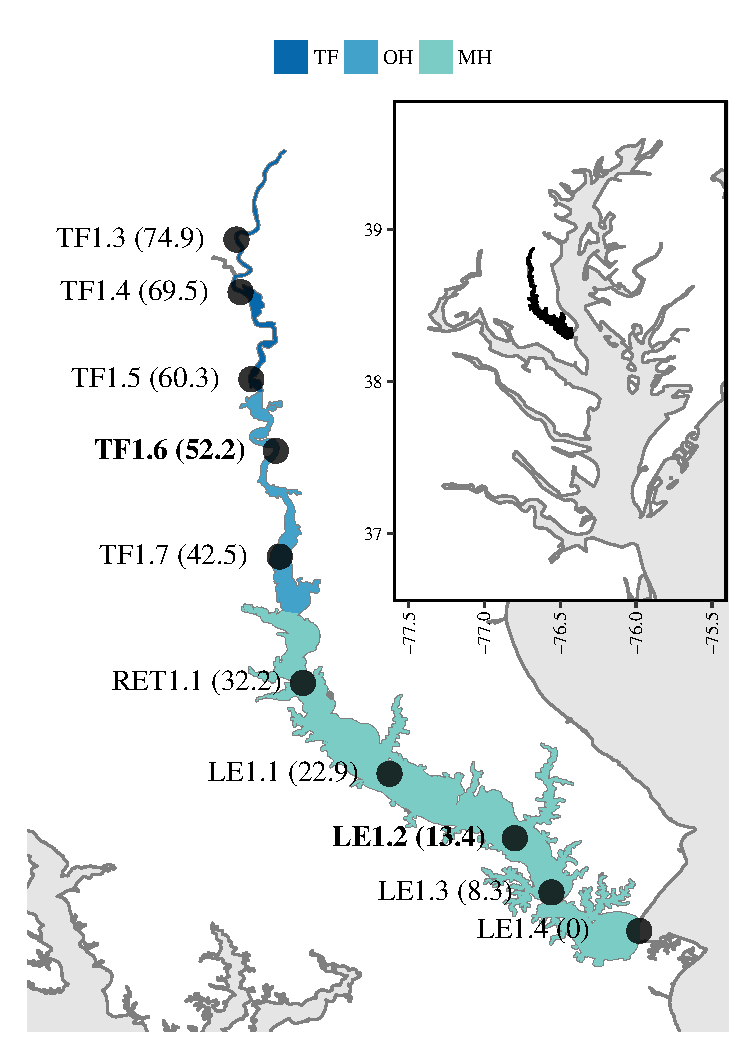
\includegraphics[width = \textwidth]{fig/patux_map.pdf}
\end{column}
\begin{column}{0.65\textwidth}
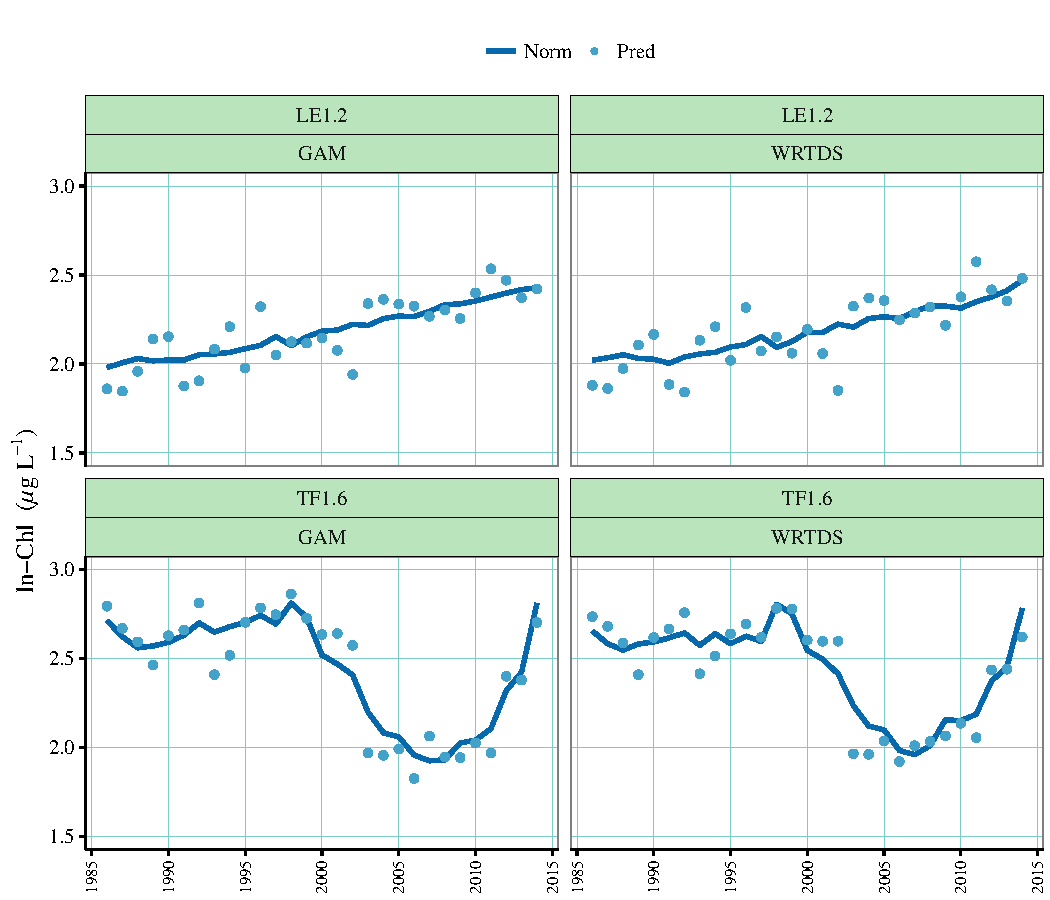
\includegraphics[width = \textwidth]{fig/predann.pdf}
\end{column}
\end{columns}
\end{frame}



%%%%%%
\begin{frame}{\textbf{Conclusions}}{\textbf{Lessons for monitoring and future work}}
DO time series and ecosystem metabolism \cite{Beck15b}
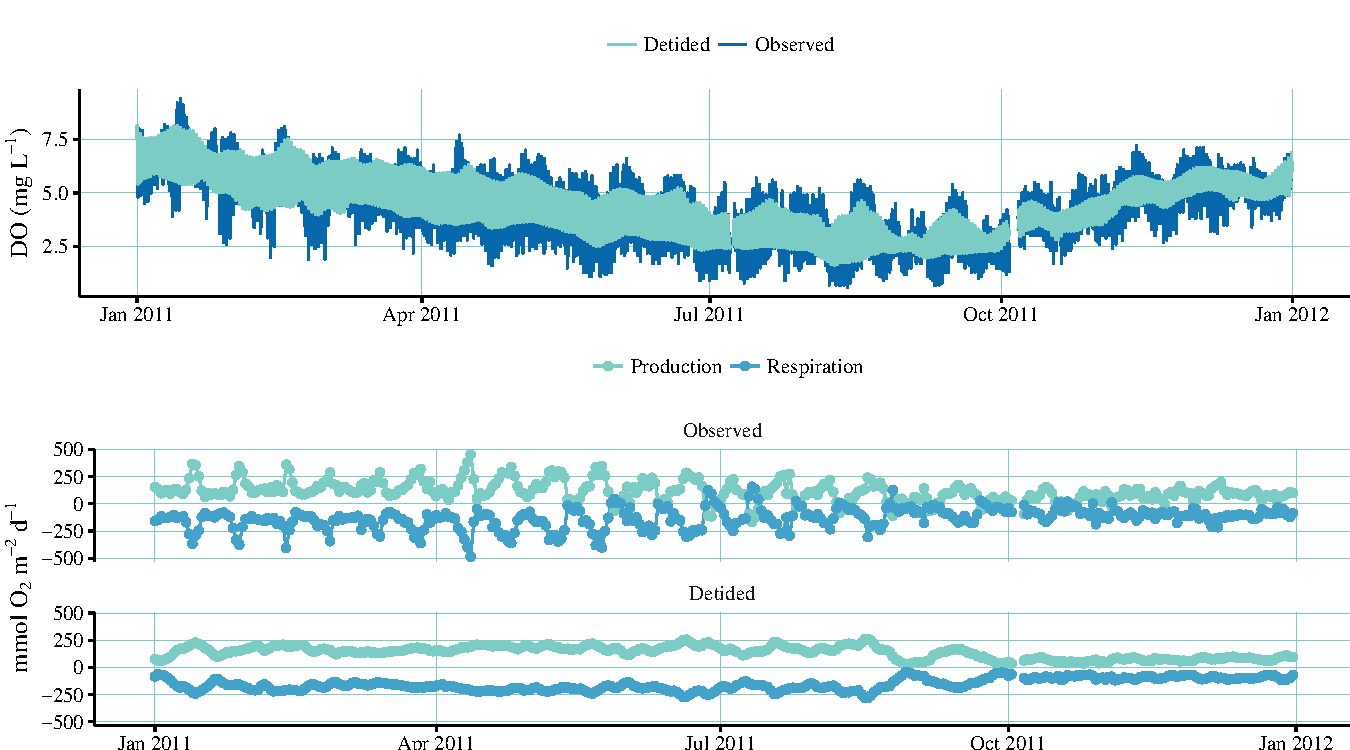
\includegraphics[width = \textwidth]{fig/metex.pdf}
\end{frame}

%%%%%%
\begin{frame}{\textbf{Conclusions}}{\textbf{Lessons for monitoring and future work}}
Data management and analysis tools
\begin{center}
\fbox{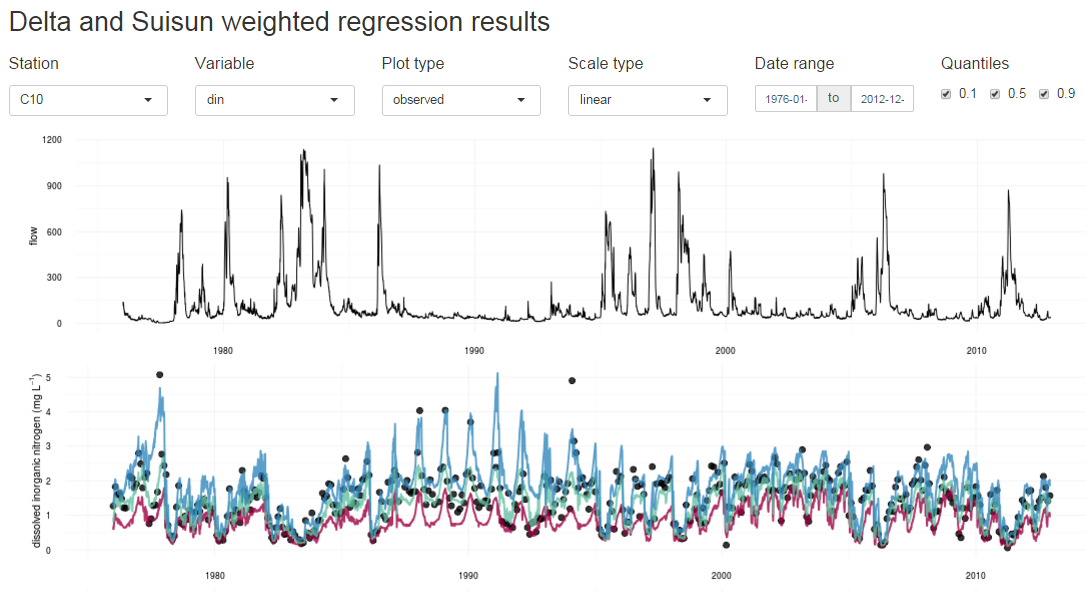
\includegraphics[width = 0.9\textwidth]{fig/shinyex.png}}
\end{center}
\end{frame}

%%%%%%
\begin{frame}
Acknowledgments and contact info:\\~\\
\begin{columns}
\begin{column}{0.9\textwidth}
{\footnotesize
Research staff and employees at USEPA Gulf Ecology Division, San Francisco Estuary Institute \\~\\
David Senn, Phil Bresnahan, Emily Novick, James D. Hagy III, Thomas Jabusch
}
\end{column}
\end{columns}
\vfill
\begin{columns}
\begin{column}{0.5\textwidth}
\begin{center}

\includegraphics[width=0.7\linewidth]{fig/titlegraphic.png}
\end{center}
\end{column}
\begin{column}{0.5\textwidth}
\scriptsize
\begin{center}
\href{mailto:beck.marcus@epa.gov}{beck.marcus@epa.gov} \\~\\
Github @fawda123 \\~\\
Phone: 8509342480
\end{center}
\end{column}
\end{columns}
\vfill
Links:\\~\\
\begin{columns}
\begin{column}{0.9\textwidth}
\scriptsize
This presentation: \href{https://github.com/fawda123/sfei_pres}{\url{https://github.com/fawda123/sfei\_pres}}

Shiny app: \href{https://beckmw.shinyapps.io/sf_trends/}{\url{https://beckmw.shinyapps.io/sf_trends/}}

Detailed results: \href{http://fawda123.github.io/sf_trends/README}{\url{http://fawda123.github.io/sf\_trends/README}}
\end{column}
\end{columns}
\end{frame}

%%%%%%
\section{References}
\begin{frame}[t]{\textbf{References}}
\tiny
\setbeamertemplate{bibliography item}{}
\bibliographystyle{apalike_mine}
\bibliography{refs}
\end{frame}

\end{document}
